% mycsrf 'for beeing included' snippet template
%
% (c) Karsten Reincke, Frankfurt a.M. 2012, ff.
%
% This text is licensed under the Creative Commons Attribution 3.0 Germany
% License (http://creativecommons.org/licenses/by/3.0/de/): Feel free to share
% (to copy, distribute and transmit) or to remix (to adapt) it, if you respect
% how you must attribute the work in the manner specified by the author(s):
% \newline
% In an internet based reuse please link the reused parts to mycsrf.fodina.de
% and mention the original author Karsten Reincke in a suitable manner. In a
% paper-like reuse please insert a short hint to mycsrf.fodina.de and to the
% original author, Karsten Reincke, into your preface. For normal quotations
% please use the scientific standard to cite
%


%% use all entries of the bibliography

\subsubsection{Frescobaldi ($\bigstar\bigstar\bigstar\bigstar\bigstar$)}

\label{Frescobaldi}\acc{LilyPond} 'bewirbt' \acc{Frescobaldi} als
\enquote{leichtgewichtigen} und \enquote{mächtigen LilyPond Musik- und
Texteditor mit vielen für die Arbeit mit LilyPond nützlichen Fähigkeiten}.
Besonders hervorgehoben wird \enquote{die beidseitige Verknüpfung zwischen dem
LilyPond Code und der dargestellten Musik} über den \enquote{‚point-and-click‘
per Maus}.\footcite[vgl.][\nopage wp]{LilyPond2018g} Daraus ergibt sich sofort,
was \acc{Frescobaldi} ist: ein Editor, bei dem der Komponist oder
Musikwissenschaftler \acc{LilyPond}-Code eingibt und als Feedback den
visualisierten Notentext erhält: \acc{Frescobaldi} gehört zu den
semi-graphischen Frontends.

Das Programm ist freie, unter GPL lizensierte Software, dessen Code auf Github
ge\-hos\-tet und zum Download bereitgestellt wird.\footcite[vgl.][\nopage
wp]{Frescobaldi2019a} Als Applikation wird \acc{Frescobald} auf einer
umfangreichen Site vorgestellt\footcite[vgl.][\nopage wp]{Frescobaldi2017a}, die
auch den Download und die Installation beschreibt \footcite[vgl.][\nopage
wp]{Frescobaldi2015a} und ein ausführliches 'Manual'
mitliefert.\footcite[vgl.][\nopage wp]{Frescobaldi2012a} Gängige Distributionen
enthalten entsprechende Programmpakete, sodass die aufwendigere Installation aus
den Quellen in der Regel nicht notwendig ist.\footcite[vgl.][\nopage
wp]{UbuntuFrescobaldi2016a}

\acc{Frescobaldi} vermag \acc{LilyPond}-Dateien direkt zu lesen und erlaubt den
konvertierenden Import von \acc{MusicXML}-, \acc{MIDI-} und \acc{ABC}-Dateien.
Als Export bietet sein Menue auf den ersten Blick 'nur' die Sicherung als
HTML-Seite an. Allerdings nutzt \acc{Frescobaldi} ja das ganze
\acc{LilyPond}-Backend. Das heißt, dass aus einer \acc{LilyPond}-Datei implizit
'immer' auch die korrespondierende \acc{MIDI}-Datei und die entsprechende
\acc{PDF}-Datei erzeugt werden.\footnote{Dies allerdings nur dann, wenn deren
Bildung über die in den Code eingebetteten 'Kommandos'
\texttt{{\textbackslash}midi \{ \}} bzw.
\texttt{{\textbackslash}layout \{ \}} mit angestoßen werden. In diesem Fall
werden die abgeleiteten Dateien unter gleichem Namenskern mit entsprechender
Datei-Extension neben der \texttt{.ly}-Datei abgelegt.} Initial muss das
Generieren dieser Artefakte für ein geladenes oder editiertes Musikstück über
das \acc{LilyPond}-Icon angestoßen werden. Unter der Rubrik \acc{Tools} kann man
dann eine Midiplayer einblenden lassen, der das Stück -- bei gelungener
Soundaktivierung -- hörbar macht.\footnote{In der Regel muss man
\acc{Frescobaldi} über den Dialog \acc{Edit/Prefrences/Midi} noch mitteilen,
über welches MIDI-Backendsystem es die Midi-Töne akkustisch generieren lassen
soll. Unter GNU/Linux respektive Ubuntu kann man z.B. \acc{timidity} über das
Shell-Kommando \texttt{timidity -iA} als Server starten, dessen geöffnete Ports
in dem \acc{Frescobaldi}-Dialog angezeigt werden, wenn man \acc{timidity} vor
\acc{Frescobaldi} gestartet hat.}

Seiner Natur nach kann \acc{Frescobaldi} unsere Referenzkadenz II direkt aus als
\acc{LilyPond}-Datei einlesen und auch unmittelbar unsere kleine
Zusatzbibliothek interpretieren, über die wir die Symbole der Harmonieanalyse in
den Notentext integrieren. Sobald man einmal das \acc{LilyPond}-Icon in der
oberen Leiste angeklickt hat, werden die entsprechenden \acc{Midi-} und die
\acc{PDF}-Dateien generiert und angezeigt:

\begin{center}
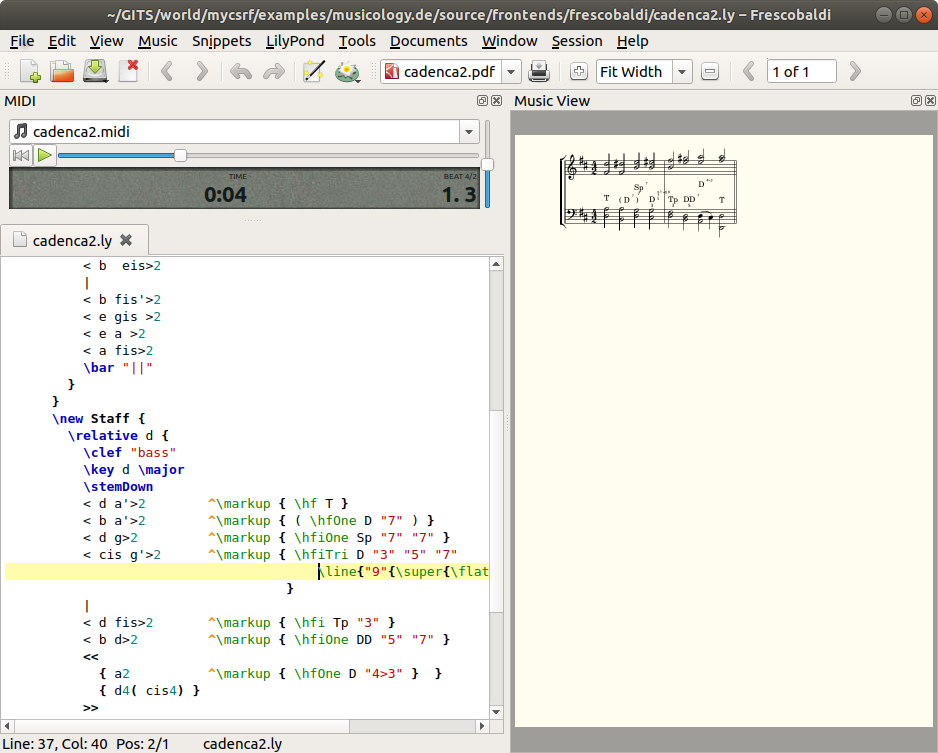
\includegraphics[width=0.9\textwidth]{frontends/frescobaldi/frescobaldi-cadenca2-300dpi.png}
\end{center}

Auf der linken unteren Seite editiert man den \acc{LilyPond}-Text, unterstützt
durch ein gelungenes Syntaxhighlighting und durch Menue-Befehle, die komplexere
Eingaben zusammenfassen. Über diesem Eingabefenster erscheint das Frontend zum
Midi-Player, wenn man diesen über die Rubrik 'Tools' aktiviert hat. Und rechts
daneben wird das generiert PDF angezeigt.

Wenn wir \acc{Elysium} mit vier Sternen ausgezeichnet haben, dann ist es nur
fair, an \acc{Frescobaldi} fünf Sterne zu vergeben: Beide Systeme gehören zur den
semi-graphischen Editoren, beide nutzen dasselbe Backend und dasselbe
Arbeitsprinzip. \acc{Frescobalid} unterstützt seinen Nutzer allerdings ein wenig
eleganter und zielgerichteter.
% this is only inserted to eject fault messages in texlipse
%\bibliography{../bib/literature}
